\section{Classificação de um triângulo}

\begin{frame}[fragile]{Classificação de acordo com as medidas dos lados}

    \begin{itemize}
        \item Sejam $a, b, c$ as medidas dos três lados de um triângulo $T$
        \pause

        \item $T$ é dito equilátero se $a = b = c$
        \pause

        \item Se dois lados tem medidas iguais e o terceiro tem medida diferente, $T$ é dito
            isóceles
        \pause

        \item Se $a \neq b\neq c$ o triângulo $T$ é denominado escaleno

    \end{itemize}

\end{frame}

\begin{frame}[fragile]{Implementação da classificação por medidas dos lados}
    \inputcode{cpp}{codes/classification_by_sides.cpp}
\end{frame}

\begin{frame}[fragile]{Classificação de acordo com as medidas dos ângulos internos}

    \begin{itemize}
        \item Sejam $\alpha, \beta, \gamma$ os ângulos internos de um triângulo $T$
        \pause

        \item Se um destes três ângulos for igual a 90\textdegree, $T$ é dito retângulo
        \pause

        \item Se um destes três ângulos for maior do que 90\textdegree, $T$ é denominado obtusângulo
        \pause

        \item Se $\alpha, \beta, \gamma <$ 90\textdegree, $T$ é chamado acutângulo 
        \pause

        \item Importante: $\alpha + \beta + \gamma =$ 180\textdegree
    \end{itemize}
        \pause

    \begin{figure}
        \centering

        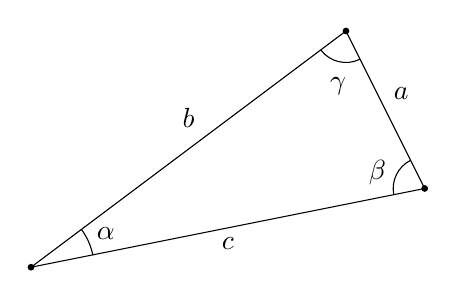
\begin{tikzpicture}
            \draw (0, 0) -- (4, 3) -- (5, 1) -- (0, 0);
            \draw[fill] (0, 0) circle [radius=1pt];
            \draw[fill] (4, 3) circle [radius=1pt];
            \draw[fill] (5, 1) circle [radius=1pt];

            \draw ({0 + 0.8*cos(11)}, {0 + 0.8*sin(11)}) arc [radius=0.8, start angle=11, delta angle=26];
            \draw ({5 + 0.4*cos(117)}, {1 + 0.4*sin(117)}) arc [radius=0.4, start angle=117, delta angle=73];
            \draw ({4 + 0.4*cos(217)}, {3 + 0.4*sin(217)}) arc [radius=0.4, start angle=217, delta angle=79];
            \node at (0.95, 0.43) { $\alpha$ };
            \node at (4.4, 1.2) { $\beta$ };
            \node at (3.9, 2.3) { $\gamma$ };

            \node at (4.7, 2.2) { $a$ };
            \node at (2, 1.9) { $b$ };
            \node at (2.5, 0.3) { $c$ };

        \end{tikzpicture}

    \end{figure}

\end{frame}

\begin{frame}[fragile]{Relação entre medidas dos lados e ângulos}

    \begin{itemize}
        \item A Lei dos Cossenos nos diz que
        \[
            a^2 = b^2 + c^2 - 2bc\cos \alpha,
        \]
        \pause
        
        \item Esta lei permite determinar o ângulo oposto ao um lado escolhido:
        \[
            \alpha = \cos^{-1} \left(\frac{b^2 + c^2 - a^2}{2bc}\right)
        \]
        \pause
        
        \item Observe que, se $\alpha =$ 90\textdegree, a Lei dos Cossenos se reduz ao 
            Teorema de Pitágoras
        \pause

        \item A Lei dos Senos também relaciona lados e ângulos, com o bônus de permitir 
            determinar o raio $R$ do círculo que circunscreve o triângulo:
        \[
            \frac{a}{\sin \alpha} = \frac{b}{\sin \beta} = \frac{c}{\sin \gamma} = 2R
        \]
    \end{itemize}

\end{frame}

\begin{frame}[fragile]{Implementação da classificação por ângulos internos}
    \inputsnippet{cpp}{1}{21}{classification_by_angles.cpp}
\end{frame}

\begin{frame}[fragile]{Implementação da classificação por ângulos internos}
    \inputsnippet{cpp}{22}{42}{classification_by_angles.cpp}
\end{frame}
